\section{Data} \label{sec:data}
We fit neural networks to a subset of the TIDIGITS dataset. These data, collected by Texas Instruments, contain audio files of over 300 speakers reciting the digits ``zero'' (and ``oh'') through to ``nine'' a number of times and in a variety of combinations. The dataset includes men, women, and children speaking in a range of accents. The subset we used includes just ten speakers, five men and five women, who repeat each of digit, in isolation, just twice, for ww recorded samples per speaker. While the data were originally recorded at 20kHz, our subset is compressed to 8kHz. We split the data into a training set (consisting of three male and three female speakers) and a test set (two male and two female). In all, this gives 132 samples in the training set and 88 samples for the test set.

 

%\subsection{Data preprocessing}
We applied a number of transformations to the data prior to analysis:
\begin{itemize}
\item \textbf{Normalising} We normalised each of the \texttt{.wav} files to mean 0, standard deviation 1.

\item \textbf{Cropping and padding} As the data were not uniformly padded with silence, we cropped each recording to remove silence at both the beginning and end of the audio file. We then padded the audio files with silence at each end to ensure the files were of the same length with the signal centred in time.

\item \textbf{Mel-frequency spectral coefficients}
The Mel-frequency cepstral coefficients (MFCC) representation of a sound is often used in speech recognition. The MFCC aims to more-closely approximate the human auditory system as frequency bands are equally spaced on the mel scale. 

The MFCC can be derived as follows:
\begin{itemize}
\item Take the Fourier transform across a window of the signal
\item Convert the powers of the spectrum onto the mel scale
\item Take the log of these powers
\item Take the discrete cosine transformation of these
\item The MFCC are the amplitudes of the resulting spectrum.
\end{itemize}
\end{itemize}

%Following from \cite{abdel2014convolutional} we use the MFSC features which use the log-energy computed from the mel-frequency spectral coefficients, which preserves locality in frequency and time.

We follow the model of \cite{abdel2014convolutional} wherein we first extract a two-dimensional spectrogram-like representation of the speech. We then apply a convolutional neural network to map this representation to a label. The representation used is simply a spectrogram which has been projected onto a log-frequency basis.

A spectrogram is a two dimensional representation of an audio waveform, often used to visualize speech and music. It expresses time in the horizontal axis and frequency in the vertical axis. Figure~\ref{fig:waveform} and \ref{fig:spectrogram} shows an example of this correspondence. In the example of Figure~\ref{fig:waveform} and in our experiments, the audio is sampled at 8kHz, and the frames of the spectrogram cover 256 samples (32ms) beginning every 32 samples (4ms).

Using the spectrogram we can read how the frequencies of the audio change over time. Each column of pixels in the spectrogram is the discrete Fourier transform of a ``frame'' - a short contiguous time slice of the waveform. These frames are equally spaced and of equal length, and are ordered by increasing time. The frames can overlap to create a smoother spectrogram. Each row of pixels in the spectrogram represents a frequency: the lowest row represents the constant component; the top row represents 4000 Hz (half the sampling frequency). The rows between are spaced linearly in the frequency space. The light-coloured bands we see in the spectrogram are the regions of high energy - these bands give some sense of the quality of the audio tone, and of its pitch.

The linear spacing of the frequency representation is not representative of human auditory perception, as humans hear multiplicative differencies in frequency as equivalent throughout the auditory range. As such, a shift in pitch - without a change in any other quality of the sound - would create a linear shift in the log-frequency domain, but a more complicated transformation in the spectrogram.

As such, we transform the spectrogram by mapping each column onto a log-frequency basis. These bases are spaced evenly in the mel scale; a mel is equivalent to $c \log(1 + f / 700)$ where $c$ is some constant and $f$ is the frequency in Hz. See Figure~\ref{fig:mfsc}, which is the mel-frequency transformation of the spectrogram in Figure~\ref{fig:spectrogram}.


\begin{figure}
\centering
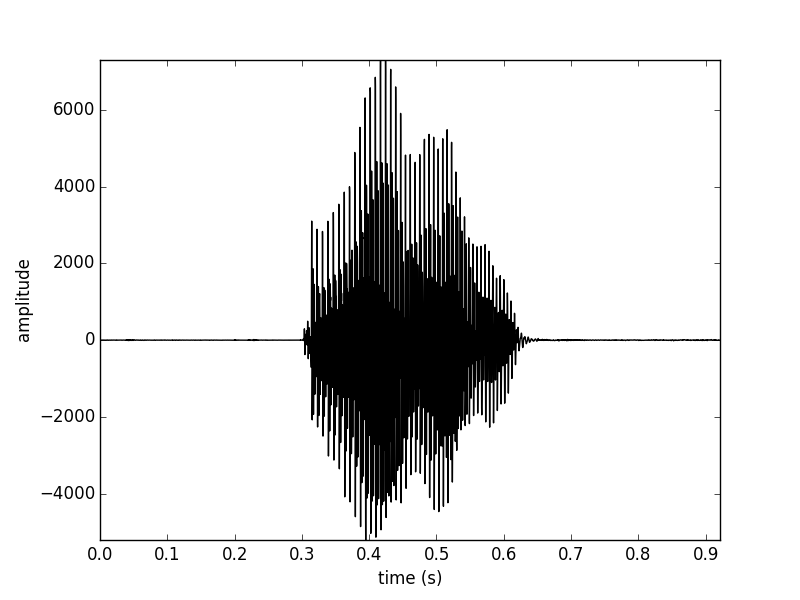
\includegraphics[width=0.8\textwidth]{waveform.png}
\caption{Waveform of the spoken word ``zero''. Cropped from the original and padded to a set length.}
\label{fig:waveform}
\end{figure}


\begin{figure}
\centering
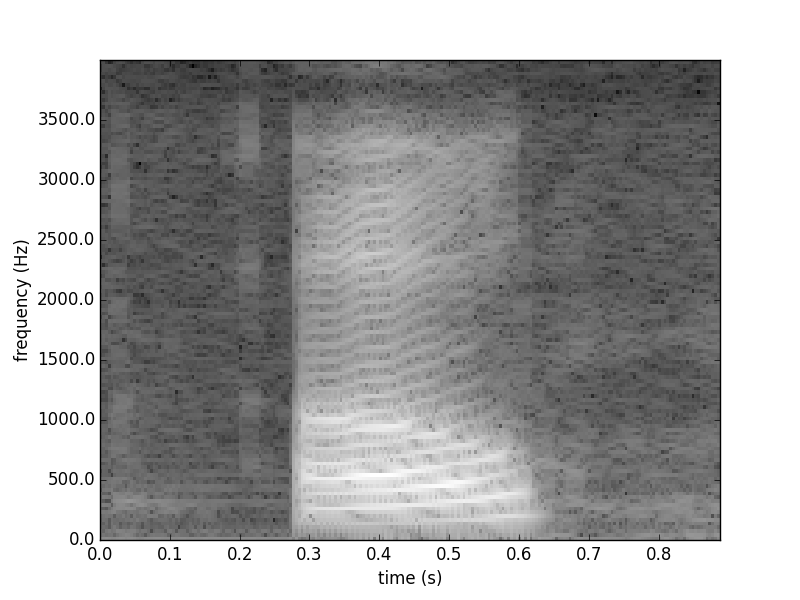
\includegraphics[width=0.8\textwidth]{spectrogram.png}
\caption{Spectrogram corresponding to the waveform in Figure~\ref{fig:waveform}.}
\label{fig:spectrogram}
\end{figure}



%\begin{figure}
%\centering
%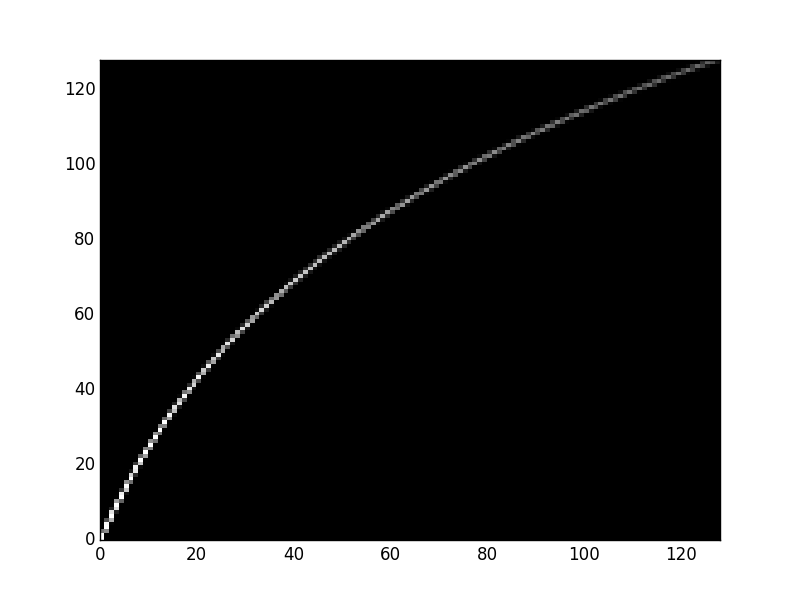
\includegraphics[width=0.8\textwidth]{mel_basis.png}
%\caption{}
%\label{fig:mel_basis}
%\end{figure}


\begin{figure}
\centering
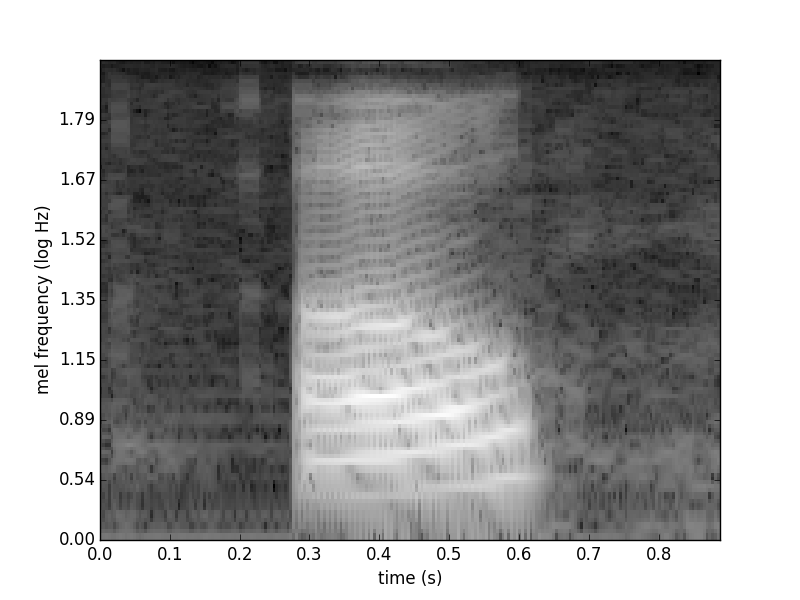
\includegraphics[width=0.8\textwidth]{mfsc.png}
\caption{Mel-frequency basis representation of the spectrogram in Figure~\ref{fig:spectrogram}. The high energy bands in the lower frequencies are spread further apart, while the high frequency bands are now closer.}
\label{fig:mfsc}
\end{figure}
















